\documentclass[a4paper, 11pt, titlepage]{article}
\usepackage{fancyhdr}
\usepackage{graphicx}
\usepackage{imakeidx}
\usepackage{makeidx}
\usepackage{mathtools}
\usepackage[spanish]{babel}
\usepackage{eurosym}
\usepackage{hyperref}
\usepackage{amssymb}
\usepackage{listings}
\usepackage{xcolor}
\usepackage{mathtools}
\usepackage{blkarray, bigstrut}
\usepackage{stackrel} 

\title{Estructura de computadores}
\author{Francisco Javier Balón Aguilar}

\begin{document}

\maketitle
\renewcommand{\contentsname}{Índice}
\tableofcontents
\newpage

\section{Unidad Central de Proceso (CPU)}\label{cpu}

    \subsection{Máquina de Von Neumann}

        La máquina de Von Neumann (1945) es un modelo computacional teórico referencia para 
        el diseño de arquitecturas de ordenadores.

        El modelo propone una unidad central de proceso (véase sección \ref{cpu}), que controla y gobierna la lógica 
        de la máquina, una memoria (véase sección \ref{memoria}) que contendrá instrucciones y datos, una unidad de entrada
        y salida (véase sección \ref{entradasalida}) que gestionará las entradas y salida de resultados, y un conjunto de periféricos.

        \begin{figure}[htp]
            \centering
            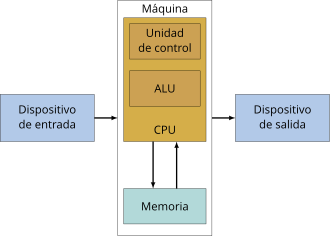
\includegraphics[width=0.7\textwidth]{resources/vonneumann.png}
            \caption{Diagrama del modelo de arquitectura Von Neumann.}
            \label{vonneumann}
        \end{figure}

        El modelo presentado, se orienta al
        procesado de información, requiriendo dos elementos: los datos y la lógica a aplicar 
        con ellos.

        Como características generales de todas las máquinas basadas en el modelo de Von Neumann, 
        podríamos citar:

        \begin{itemize}
            \item Uso de componentes lógicos básicos, tal y como puertas lógicas, transistores... 
            \item Configuración de uso general de funciones lógico-aritméticas.
            \item Uso de memoria, tanto para el almacenamiento de datos como de instrucciones.
            \item Uso de circuito secuencial (unidad de control). Véase la sección \ref{unidadcontrol} 
            para mayor detalle.
            \item Provisión de instrucciones y datos.
        \end{itemize}

        Tal y como se observa en la figura \ref{vonneumann}, los elementos que lo componen son:

        \subsubsection{Memoria en la máquina de Von Neumann}

            La memoria está compuesta por un conjunto de celdas de la misma longitud (mismo número de
            bits), que almacenan tanto datos como instrucciones, siendo cada una de ellas identificada 
            una dirección unívoca (dirección de memoria). El sistema puede leer la información contenida 
            en ellas y escribir nuevos datos.

        \subsubsection{Unidad aritmético-lógica (ALU) en la máquina de Von Neumann}

            En esta unidad se realizan las operaciones básicas lógicas y de tipo aritmético, 
            tales como sumar, restar, AND, OR, XOR...

            Los datos se obtienen de la memoria principal y se escriben en la misma los resultados 
            finales. Los resultados intermedios se almacenan temporalmente en registros de la propia 
            ALU.

        \subsubsection{Unidad de Control (UC) en la máquina de Von Neumann}

            Es la encargada de ejecutar las instrucciones almacenadas en memoria, procediendo previamente 
            a su captura y decodificación para después interpretando el tipo de instrucción a ejecutar y 
            generando posteriormente las señales de control para su interpretación.
            
        \subsubsection{Unidad de Entrada y Salida en la máquina de Von Neumann}

            Se encarga de gestionarla transferencia de información entre los periféricos y la unidad 
            central de proceso.

        \subsubsection{Buses en la máquina de Von Neumann}

            Son los elementos que interconectan los componentes. Su objetivo es por tanto la transferencia 
            de información, bien sean datos o señales entre los diferentes dispositivos.

            Por lo general distinguimos tres tipos de buses:

            \begin{itemize}
                \item \textbf{Buses de datos}.
                \item \textbf{Buses de control}.
                \item \textbf{Buses de direcciones}.
            \end{itemize}

    \subsection{Ciclo Básico de Instrucciones}

        Como ya se ha visto, es la unidad de control la encargada de ejecutar las instrucciones que procedan 
        en cada momento, siguiendo una serie de pasos básicos (véase también la figura \ref{cicloinstruccion}):

        \begin{enumerate}
            \item Pasar una instrucción de memoria a la unidad de control.
            \item Interpretar (decodificar) la instrucción.
            \item Ejecutar la instrucción:
            \begin{enumerate}
                \item Pasando los datos necesarios, accediendo a memoria con esas direcciones de los datos 
                calculadas para llevar los datos a la ALU y proveer registros en la ALU para su almacenamiento.
                \item Generando señales de control para la ejecución de las operaciones.
                \item Generando el resultado, ya sea en la ALU (si hay datos) o en la unidad de control (si no 
                existen datos).
            \end{enumerate}
            \item Ejecutar --si existe-- la siguiente instrucción.
        \end{enumerate}

        \begin{figure}[htp]
            \centering
            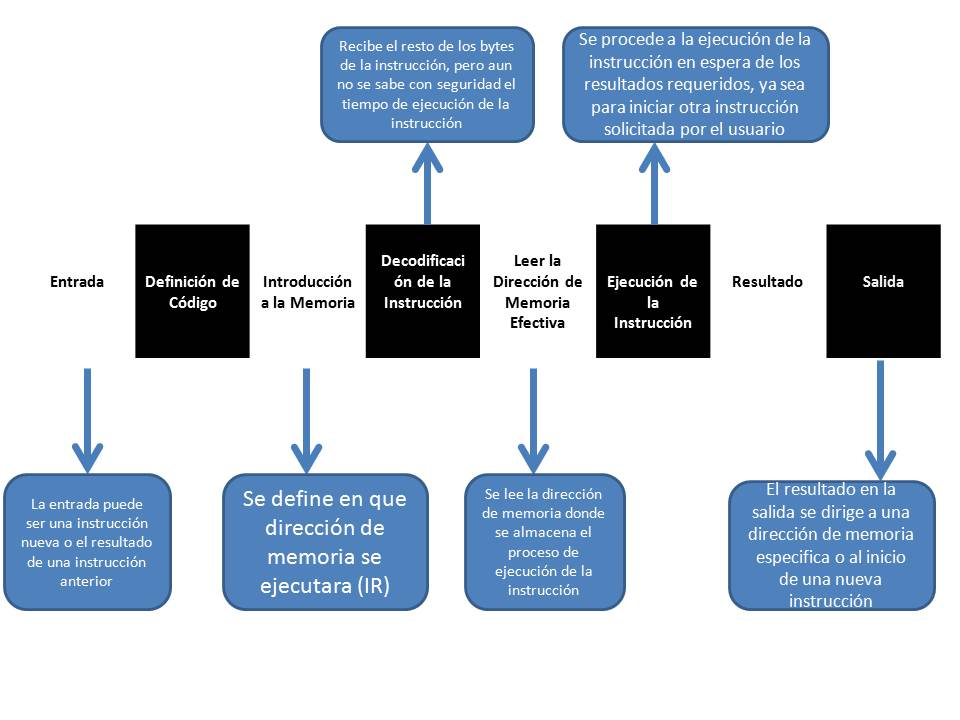
\includegraphics[width=0.8\textwidth]{resources/cicloinstruccion.jpg}
            \caption{Esquema del ciclo de instrucción.}
            \label{cicloinstruccion}
        \end{figure}

        \subsubsection{Registros y operaciones básicas}

            Los registros son un conjunto de biestables (bits) que se utilizan como almacén y que realizan las
            siguientes operaciones comunes:

            \begin{itemize}
                \item \textbf{Lectura}.
                \item \textbf{Escritura}.
                \item \textbf{Transferencia}. $(RA)\rightarrow RB$
                \item \textbf{Incremento} (INC). $(R1) + 1 \rightarrow R$
                \item \textbf{Decremento} (DEC). $(R1)-1 \rightarrow R$
                \item \textbf{Complemento} (CMP). $1 = 0; 0=1$
                \item \textbf{Reset} (RES).
                \item \textbf{Set} (SET).
            \end{itemize}

        \subsubsection{Instrucciones, $\mu$operaciones y $\mu$órdenes}

            Un programa se compone de una serie de instrucciones, compuestas a su vez en ciclos (fases),
            $\mu$operaciones y $\mu$órdenes.

            Una instrucción se compone de cuatro ciclos; de captación, de indirección, de ejecución y 
            de interrupción. Cada ciclo comprende la realización de una serie de pasos; y para ejecutar 
            cada uno de ellos se deben realizar una serie de operaciones atómicas o $\mu$operaciones.

            Cada conjunto de $\mu$órdenes que se emite en un ciclo de reloj de la unidad de control, se 
            denomina $\mu$instrucción.

            Una instrucción en lenguaje máquina se divide en $\mu$instrucciones.

        \subsubsection{Tipo de instrucciones}

            \begin{enumerate}
                \item Pueden ser de procesado de datos, donde se realicen operaciones aritméticas u operaciones 
                lógicas.
                \item Pueden llevar a cabo instrucciones de transferencia de información, bidireccionalmente 
                entre la memoria y el módulo de entrada y salida, o entre la memoria y los registros de la CPU.
                \item Pueden ser de control de flujo, como comprobación de un resultado o la alteración de la secuencia 
                normal.
            \end{enumerate}

            La representación de las instrucciones se realiza a através de una cadena de bits, cuyo conjunto se 
            divide en campos, y cada campo indica un tipo de información; de tal forma que el formato de la 
            instrucción determina el número de campos que debe tener esa instrucción, la longitud de cada campo, 
            su contenido y la posición del campo dentro de la cadena de bits (véase figura \ref{formatoinstruccion}).

            \begin{figure}[htp]
                \centering
                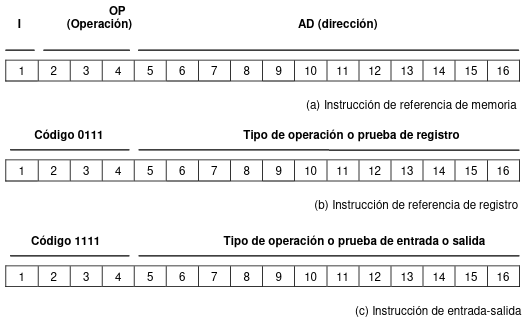
\includegraphics[width=0.8\textwidth]{resources/formatoinstruccion.png}
                \caption{Ejemplo de formato de instrucción.}
                \label{formatoinstruccion}
            \end{figure}

            Dependiendo del tipo de instrucción que se procese, puede manejar unos tipos de datos diferentes, siendo:

            \begin{itemize}
                \item Direcciones.
                \item Números.
                \item Caracteres.
                \item Datos lógicos (cadenas de $n$ bits manejados de forma individual).
                \item Estructura de datos.
            \end{itemize}

            Otro aspecto a considerar dentro de las instrucciones es el tipo de operación que deben desarrollar, 
            clasificadas en:

            \begin{itemize}
                \item De transferencia.
                \item Aritméricas.
                \item Lógicas.
                \item De conversión.
                \item De control de flujo.
                \item Instrucciones de control del sistema.
            \end{itemize}

    \subsection{La Unidad de Control}\label{unidadcontrol}

        La unidad de control es un circuito secuencial cuyo objetivo es captar, interpretar y ejecutar 
        las instrucciones almacenadas en memoria. Está formada por una serie de registros que gobiernan 
        su funcionamiento, siendo los más importantes los registros de control y de estado, que se utilizan 
        para mantener el control de los procesos. De entre ellos, los más importantes son:

        \begin{itemize}
            \item Registro contador de programa (CP), que contiene la dirección de la siguiente instrucción 
            a ejecutar.
            \item Registro de instrucción (RI), que contiene la instrucción captada más recientemente.
        \end{itemize}

        Dentro de cada instrucción debe existir un código de operación, que contenga el tipo de operación a 
        realizar (CO), la longitud de la instrucción (LI), el modo de direccionamiento (MD) y el número de 
        operandos.

        El campo de direcciones (CD) puede contener un dato inmediato, una dirección inmediata o una dirección 
        parcial. R1 y R2 es la identificación de los registros utilizaods en la instrucción.

        La dirección final DF es la dirección efectiva cuyo contenido es el dato que se quiere procesar, obtenido
        mediante el contenido de CD.

        \begin{itemize}
            \item \textbf{Registro de estado}. Contiene la información generada por el sistema.
            \item \textbf{Registro de estado de un programa}. Contiene información de estado del sistema y códigos 
            de condición sobre la última operación realizada en la ALU.
            \item \textbf{Registro de interrupciones}. Contiene información sobre los dispositivos que han producido 
            una interrupción.
            \item \textbf{Registro de punteros}. Contiene direcciones específicas de procesos en segmentación, paginación\dots
        \end{itemize}

        Por otro lado, en la unidad de control debe existir un decodificador, un controlador y un reloj del 
        sistema \footnote{
            El reloj de la CPU es el que genera los pulsos de reloj, que marcan la velocidad del microprocesador. Un ciclo 
            de CPU es un pulso electromagnético. En función del tipo de instrucción, se completará un número de pulsos 
            determinados.
        } (véase figura \ref{unidadcontrol} para mayor detalle).

        \begin{figure}[htp]
            \centering
            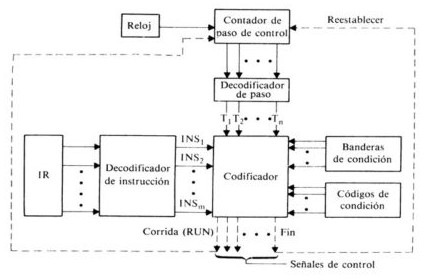
\includegraphics[width=0.8\textwidth]{resources/unidadcontrol.jpg}
            \caption{Esquema de la unidad de control.}
            \label{unidadcontrol}
        \end{figure}

        Como salida, la unidad de control genera las microórdenes a través de los buses dirigidos a todos los 
        componentes del sistema, trasferiendo información entre ellos, y por lo tanto la ejecución de $\mu$operaciones.

    \subsection{Unidad Aritmético-Lógica}

        Es un circuito combinacional que se encarga de realizar las operaciones con los datos, teniendo unas 
        entradas (correspondientes a las $\mu$órdenes existentes) que indican el tipo de operación a realizar 
        con los datos de entrada (véase figura \ref{alu}).

        \begin{figure}[htp]
            \centering
            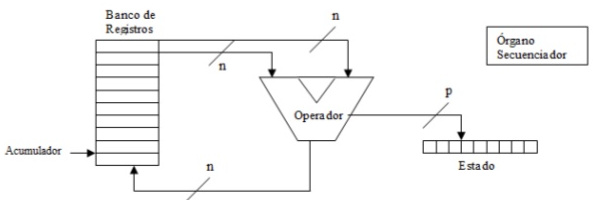
\includegraphics[width=0.8\textwidth]{resources/alu.jpg}
            \caption{Esquema de la unidad aritmético-lógica.}
            \label{alu}
        \end{figure}

        Consta de una base de registros para realizar las operaciones necesarias; siendo éstos de propósito general 
        y visibles al programador de lenguaje máquina.

        \subsubsection{Modos de direccionamiento}

            Son los procesos que permiten conocer la localización de una instrucción o dato. Los modos de direccionamiento 
            dependen de la arquitectura del computador. De entre los más comunes encontramos:

            \paragraph{Direccionamiento inmediato} Se produce cuando el CD contiene un dato inmediato, y no la 
            dirección en la que se encuentra el dato. Si la longitud de la instrucción es P1 (una palabra) se produce 
            1 acceso a memoria; si por el contrario es P2 se producen 2 accesos a memoria (captura y ejecución).

            \paragraph{Direccionamiento directo} Se produce cuando el CD contiene la dirección del dato a recuperar.
            Si la longitud es P1, se producen 2 accesos a memoria (captura y ejecución); si por el contrario 
            la longitud es P2 se producen 3 accesos a memoria (1 en captura y 2 en ejecución); si la longitud es P3 
            (instrucciones con 2 operandos) se producen 5 accesos a memoria (1 en captura, 2 en ejecución y 2 en 
            recuperación del dato contenido en las direcciones CD1 y CD2).

            \paragraph{Direccionamiento indirecto} Se produce cuando el CD contiene una dirección cuyo contenido es otra 
            dirección de memoria con el dato.

            \paragraph{Direccionamiento mediante registros} En él, existe un trabajo (RT) que contiene el dato a procesar 
            o su dirección. El código MD (modo de direccionamiento) indica el registro utilizado y el tipo de contenido.

            \paragraph{Direccionamiento con desplazamiento} Siempre se referencian datos en la memoria principal; para obtener 
            el CD de memoria es preciso efectuar una suma.

            \paragraph{Direccionamiento por pilas} Se define su tamaño y permite incluir elementos en ella [la pila] 
            hasta el valor máximo.

    \subsection{Arquitectura CISC vs RISC}

        \subsubsection{Introducción a la ISA}

            Una ISA (Instruction Set Architecture) o arquitectura del conjunto de instrucciones es el repertorio de 
            instrucciones\footnote{
                Una instrucción no es más que un segmento de código que contiene implícita una operación que la CPU debe 
                realizar.
            } que puede entender y ejecutar la unidad de control de una determinada CPU. Eso no solo 
            incluye las instrucciones (tipos, codificación,…) comprensibles por la CPU, sino también el tipo de 
            datos aceptados de forma nativa, endianness, tamaño y cantidad de registros, arquitectura de la memoria, 
            e interrupciones/excepciones, extensiones, branching, etc. 

            En otras palabras, podríamos considerar a la ISA como la capa visible al programador a bajo nivel.

            Una ISA puede ser implementada (cómo se van a procesar o tratar sus instrucciones y datos) sobre lo que se 
            conoce como \textit{microarquitectura}\footnote{
                No hay que confundir el término microarquitectura ($\mu$arch) con arquitectura. Ésta segunda engloba 
                tanto la ISA como la microarquitectura, además de otros elementos y aspectos más amplios dentro del 
                sistema en conjunto del computador, que son estudiados en esta asignatura.
            }. Para ello será necesario contar con una serie de unidades funcionales
            (multiplexores, ALU, FPU, registros, unidad de control y demás circuitería).

            Diferentes microarquitecturas pueden ser compatibles con una misma ISA, pero una microarquitectura no 
            podrá procesar otra ISA diferente para la que fue diseñada; al menos de forma nativa.

            Dentro de las ISAs encontramos varios tipos, que diferenciándolas \textit{grosso modo} en el tamaño 
            del repertorio de instrucciones y longitud obtenemos:

        \subsubsection{CISC}
        
            Son las siglas de Complex Instruction Set Computer, es decir, un modelo de 
            ISA complejo. Se compone de instrucciones largas, gran número de ellas y que pueden realizar 
            bastantes operaciones complejas con los oprandos situados en la memoria o registros. Aparecieron 
            antes que otros tipos, por eso CISC es un retrónimo. Algunos ejemplos de CISC son IBM System/370, 
            Zilog Z80, Motorola 68k, National Semiconductor 32016, MOS Technology 6502, DEC PDP-11, DEC VAX, 
            x86 (pre-x86, x86-8, x86-16, x86-32, x86-64), IBM z/Architecture, etc.

            Algunas características propias de este tipo son:

            \begin{itemize}
                \item La complejidad hace que el coste y el tiempo invertido en la implementación sea mayor.
                \item Suele tener una unidad de control microprogramada, más lenta y menos eficiente.
                \item Dispone de pocos bancos de registros de propósito general.
                \item Suelen ocupar más espacio en el silicio, lo que encarece su producción y baja el yield.
                \item Tamaño variable y largo. Gran cantidad de instrucciones, llegando a las 500 en algunos casos. 
                Necesitan varios ciclos de duración, por tanto el CPI es mayor, o lo que es lo mismo, el IPC es menor.
                \item Tenemos más cantidad de modos de direccionamiento y complejos.
                \item El tiempo de programación es menor, una de las pocas ventajas de CISC frente a RISC.
                \item El compilador no es crítico y puede ser más sencillo.
                \item El programa suele ser más compacto, ya que con pocas instrucciones complejas basta.
                \item La abstracción es alta, siendo el software algo más independiente del hardware.
            \end{itemize}

        \subsubsection{RISC}\label{risc}
        
            Son las siglas de Reduced Instruction Set Computer, es decir, un modelo de 
            ISA simple que surge para resolver algunos problemas destacados de los CISC. A finales de los 70 
            se comenzó a ver un fenómeno curioso, y es que algunas versiones de arquitecturas CISC de gama 
            baja a las que se le retiraban algunas de las instrucciones complejas para reducir costes en la 
            implementación, en vez de ir peor mejoraban su rendimiento. Por ese motivo se comienzan a diseñar 
            los primeros RISC con repertorios de instrucciones más reducidos e instrucciones simples. 
            Ejemplos son el AMD 29000, ARM, DEC Alpha, RISC-V, MIPS, HP PA-RISC, IBM PowerPC/POWER, SPARC, 
            etc.

            Algunas características propias de este tipo son:

            \begin{itemize}
                \item El tiempo de desarrollo para una microarquitectura de este tipo es más bajo y el coste más reducido.
                \item El tipo de unidad de control suele ser cableada, es decir, mucho más rápida y eficiente.
                \item Suelen tener gran cantidad de registros de propósito general.
                \item El espacio de integración es más bajo en igualdad de condiciones. Es decir, el dado o core tendrá 
                menor superficie.
                \item El tamaño de instrucciones es fija y corta. En cuanto a cantidad, suele ser reducido, normalmente 
                inferior a las 128 instrucciones. Suelen durar solo un ciclo de duración.
                \item La cantidad de modos de direccionamiento de memoria son pocos y simples.
                \item El tiempo de programación es más elevado.
                \item El compilador debe ser complejo y muy eficiente.
                \item El tamaño del programa generado es hasta un 30\% mayor al necesitar de más instrucciones 
                simples para realizar una misma tarea en comparación con CISC.
                \item La abstracción software/hardware es baja. El software está muy ligado al hardware.
            \end{itemize}

            \paragraph{}{RISC-V} Dentro de las RISC existen muchas ISAs en actual uso, entre ellas las conocidas \textit{SuperH}, \textit{ARM} 
            (con buena relación rendimiento/eficiencia energética), \textit{RISC} y \textit{MIPS} (las primeras de ellas, por 
            ello llevan el nombre de RISC), etc.

            Pero la más moderna y que merece mención especial es \textit{RISC-V}. Ésta se desarrolla sobre una licencia 
            libre (\textit{BSD}). Iniciado por Berkeley con fondos del DARP, y actualmente participan en su creación multitud 
            de miembros de la fundación

        \subsubsection{Otros tipos}

            Aunque CISC y RISC son los dos grandes tipos de ISA y más relevantes, existen otros:
            
            \begin{itemize}
                \item \textbf{ZISC} Zero Instruction Set Computer no cuenta con un conjunto de instrucciones (en el sentido 
                clásico). Se basa en la mera coincidencia de patrones, similar a los computadores analógicos donde tampoco 
                existían, aunque aquí hablamos de computadoras digitales. Ha habido pocas implementaciones de este tipo, algún 
                ejemplo sería el IBM ZISC35 o el ZISC78, e incluso algunos chips neuronales como el CM1K…
                \item \textbf{SISC} Specific Instruction Set Computer es similar a RISC, de hecho se podría catalogar como tal, 
                pero es aún más reducidopara optimizar el rendimiento para alguna aplicación específica. Empleado en algunos 
                microcontroladores y ASIPs. Un ejemplo, algunos autores dicen que el DSP TMS320 de TI (Texas Instruments) es 
                SISC y otros lo etiquetan como RISC…
                \item \textbf{VISC} Virtual Instruction Set Computer es otro tipo introducido por Soft Machines.
                \item \textbf{DISC} Dynamic Instruction Set Computer puede modificar el conjunto de instrucciones de forma dinámica 
                según la demanda o exigencias del programa. Se suele usar para FPGAs reconfigurables.
                \item \textbf{NISC} No Instruction Set Computer tiene una tecnología muy específica de compilador y se emplea en 
                CPUs de alta eficiencia para algunas aplicaciones críticas, aceleradores por hardware, etc. No necesita de ROM de 
                microcódigo, ni controladores sofisticados, ni decodificador de instrucciones, etc.
                \item \textbf{MISC} Minimal Instruction Set Computer también es un conjunto muy reducido de instrucciones, pero a
                diferencia de otros como SISC o RISC, los operandos se almacenan en la pila en vez de en los registros, reduciendo 
                así el tamaño de los operandos y simplificando al máximo la microarquitectura. Funciona rápido y la unidad de 
                decodificación de instrucciones es más pequeña.
                \item \textbf{EDGE} Explicit Data Graph Execution intenta mejorar las carencias de CISC y evitar los problemas de 
                cuello de botella. Contiene muchas instrucciones individuales en un grupo denominado hyperblock y puede ser 
                ejecutado en paralelo.
                \item \textbf{OISC} One Instruction Set Computer, también llamado URISC (Ultimate RISC). Usa solo una instruccion 
                sin limitar las aplicaciones. Sus implementaciones se usan especialmente para la enseñanza. Imagina una instrucción 
                SUBLEQ que reste el contenido de dos direcciones de memoria y almacene el resultado en otra dirección. Con esa única 
                instrucción, ejecutandola secuencialmente se podrían conseguir los equivalentes a varias instrucciones. Por ejemplo, 
                si se ejecuta SUBLEQ b, b + SUBLEQ a, Z + SUBLEQ Z, b + SUBLEQ Z, Z = MOV a, b.            
            \end{itemize}

        \subsubsection{Híbridos CISC-RISC (RISC-Like)}

            Algunos diseñadores de microarquitecturas CISC han querido obtener las ventajas de RISC sin abandonar el modelo CISC o sin 
            perjudicar a la compatibilidad del software escrito para su ISA. Eso sería el caso de x86. CISC es un modelo antiguo y con 
            carencias, pero ¿cómo pasarse a RISC sin crear una nueva ISA y sin que todo el software compatible tenga que ser compilado 
            para esta nueva arqutiectura? La solución es la hibridación.

            Uno de los primeros diseños RISC-like sería el AMD K5, que usaba la exitosa microarquitectura del 29k a la que le añadieron 
            un Front-End para traducir las CISC-x86 y posibilitando que el Back-End trabajase de forma superescalar, con ejecución fuera 
            de orden, ejecución especulativa, renombre de registros, etc., sin alterar la compatibilidad con x86.

            Actualmente, los diseños de Intel y AMD trabajan como RISC a nivel electrónico, aunque el repertorio de instrucciones sea 
            CISC.

\section{Memoria}\label{memoria}

    %\subsection{Aspectos físicos}

        Las memorias tienen una serie de características físicas a tener en cuenta:

        \begin{itemize}
            \item \textbf{Volatilidad}. Capacidad de retener o perden la información almacenada en caso de 
            corte de suministro eléctrico.
            \item \textbf{Alertabilidad}. Posibilidad de alterar el contenido de una memoria.
            \item \textbf{Permanencia de la información}. Relaciona la duración de la información almacenada.
            \item \textbf{Almacenamiento estático/dinámico}. Una memoria es estática cuando su información 
            permanece inalterable a lo largo del tiempo (véase SRAM); una memoria es dinámica cuando necesita 
            realizar un ciclo de refresco para poder retener la información que almacena (DRAM).  
        \end{itemize}

        En función del tiempo de almacenamiento mencionado, se hará distinción en la volatilidad. Por el lado volátil 
        observamos la memoria RAM dinámica (DRAM - que contiene los programas en ejecución y los datos con los que operan), 
        la memoria caché (típicamente SRAM, más rápida que DRAM pero con mayor consumo energético y menor capacidad) y los 
        registros del procesador. Estas memorias, junto a la ROM (no volátil) comprenden el denominado almacenamiento 
        primario del ordenador.

        Frente a él, el denominado almacenamiento secundario o almacenamiento masivo, que requiere el uso de buses 
        de entrada/salida para acceder a la información, usualmente no volátil. Este tipo de almacenamiento tiene un 
        tiempo de acceso mucho mayor que el primario, su capacidad de almacenamiento supera ampliamente la del almacenamiento 
        principal.

        En resumen, las características de la memoria principal son: electrónicas, con alta velocidad, tamaño limitado, 
        volátil o no volátil, imprescindible y de elevado coste. Mientras que las de la memoria secundaria son: 
        magnética u óptica, velocidad reducida en comparación, tamaño ilimitado, permanente y estática, opcional en el sistema 
        y de bajo coste.

        \begin{figure}[htp]
            \centering
            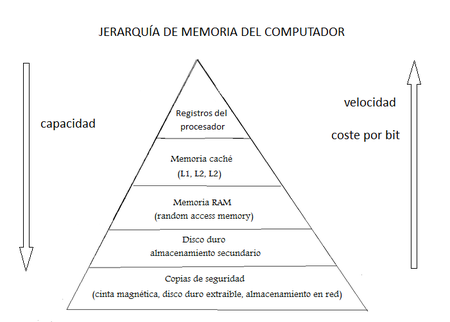
\includegraphics[width=0.8\textwidth]{resources/jerarquiamemoria.png}
            \caption{Jerarquía de memorias.}
            \label{jerarquiamemoria}
        \end{figure}

\section{Módulo de Entrada y Salida}\label{entradasalida}

    La entrada y salida de datos representa el medio de comunicación existente entre el usuario y el 
    ordenadr, logrando a su vez la eficiencia en las operaciones de E/S y minimizando el trabajo a 
    realizar a la CPU.

    Cuenta con dos elementos básicos unidos por los correspondientes buses:

    \subsection{Interfaz o controlador del periférico}

        Sistema mixto hardware/software que posibilita la comunicación entre la CPU/memoria y el 
        periférico, siendo sus principales funciones:

        \begin{itemize}
            \item Control de transferencia de datos entre dispositivo y procesador,
            \item Adaptación de longitud y formato de datos.
            \item Arbitraje de bus.
            \item Adaptación de los tiempos de transferencia de CPU y periférico.
            \item Adaptación de señales eléctricas para la conexión de un periférico.
            \item Decodificación de las órdenes provenientes del procesador.
            \item Averiguar qué dispositivo se encuentra disponible para transferir datos.
            \item Comunicación con los dispositivos.
            \item Almacenamiento temporal de datos.
            \item Detección de errores en el funcionamiento del dispositivo.
        \end{itemize}

    \subsection{Operación de entrada/salida (E/S)}

        La operación de entrada/salida se lleva a cabo de la siguiente manera:

        \begin{quote}
            \small En primer lugar, se comprueba si el dispositivo está listo, leyendo el registro 
            de estado del controlador, donde un bit indicará si puede comenzar a transferir una palabra.

            El registro de control indicará el tipo de operación a realizar, donde los distintos bits de 
            dicho registro indican cada una de las distintas acciones a llevar a cabo por el 
            periférico.

            Para comenzar una operación, el procesador debe escribir sobre los registros anteriores los 
            distintos datos de la operación a través de una dirección de E/S o memoria asignada únicamente 
            al controlador. Después, se transfiere el dato usando el registro de datos.

            Una vez concluida la transferencia debe indicarse en el registro de control.
        \end{quote}

    \subsection{Dispositivos periféricos}

        Son aquellos dispositivos que se conectan con el procesador. Éstos permiten realizar operaciones 
        de E/S en las que suelen intervenir memoria y CPU. Para conectar estos 3 componentes se utilizan 
        los siguientes buses:

        \begin{itemize}
            \item Bus de direcciones.
            \item Bus de datos.
            \item Bus de control.
        \end{itemize}

    \subsection{Tipos de entrada/salida}

        Hay 3 tipos fundamentales por los cuales puede realizarse la operación de E/S:

        \subsubsection{E/S por intrrupciones}

            La E/S se realiza mediante una rutina de atención a la interrupción, donde el dispositivo 
            indica a la CPU cuando está listo.

        \subsubsection{E/S por consulta o programada}

            Se realiza una consulta periódica al dispositivo para saber cuándo se encuentra disponible 
            para operar. Es un proceso de mayor sencillez, pero la velocidad de transferencia está limitada 
            a la velocidad que imponga la CPU. Además, existe el riesgo de sobrecarga.

        \subsubsection{E/S por acceso directo a memoria}

            El dispositivo accede directamente a memoria y se encarga de avisar a la CPU tanto del inicio 
            como del final de la tarea. La velocidad de transferencia obtenida es superior.

\section{Buses}

\end{document}